\documentclass[11pt]{scrartcl}

\usepackage[top=1in, bottom=2cm, left=1in, right=1in]{geometry}
\usepackage{graphicx}
\usepackage{amsmath}
\usepackage{subfig}

\begin{document}

\title{Final Project STAT5376}
\subtitle{Registration of hand writing speed}
\author{Li Sun}
\date{\today}
\maketitle

\noindent
1. Goal: Given 50 writing data of Chinese word 'statistical science' recording 601 times along the way. Average writing time is 6 seconds. So our data showed pen position ten times per second. Our goal is find out pen moving speed along the writing process and treat this as functions. And we need to register the 50 functions by using SRSF representation. 

\bigskip

\noindent
2. Data view\\
The data comes in a 601 by 3 matrix with x,y and z coordinates, and we will use only x and y position. z is not used. The first observation was visualized as following.\\
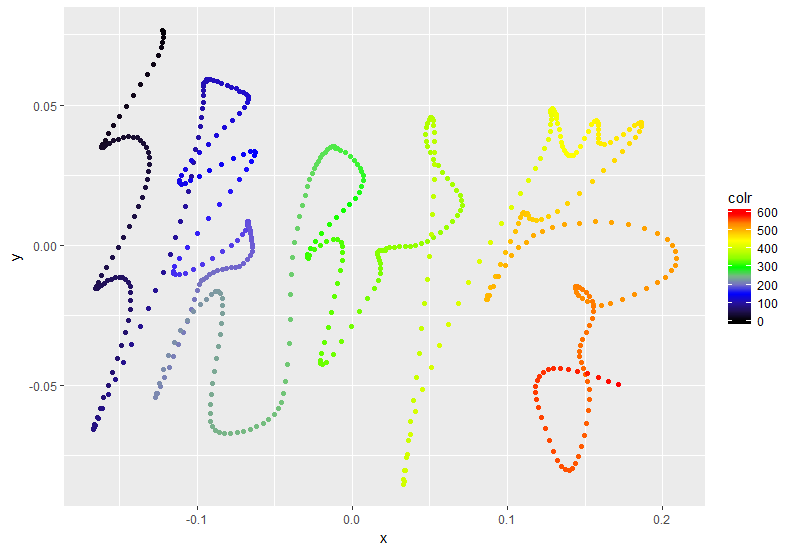
\includegraphics[scale=0.7]{fp00.png}\\
The color is t value from 0 to 600.\\
In this study, we will be focusing on the moving speed of the pen when writing these words. So I smooth x and y coordinates along the time separately as the following two figure.\\
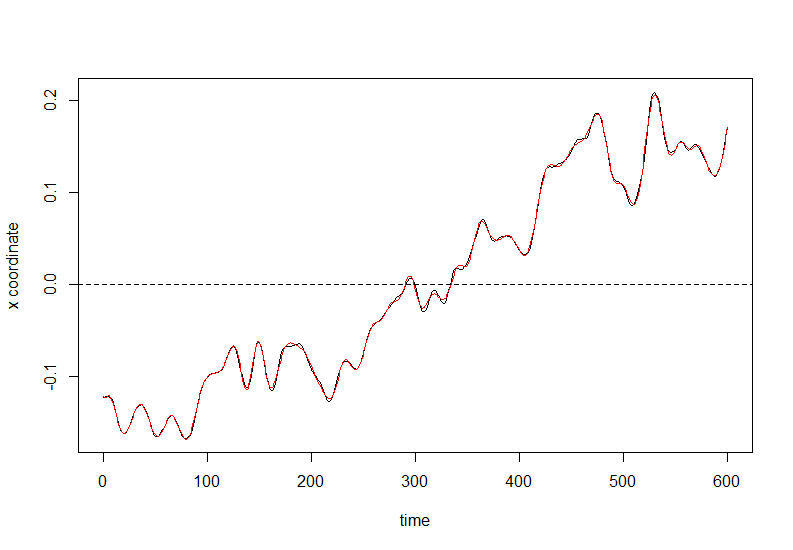
\includegraphics[scale=0.7]{fp01.png}\\
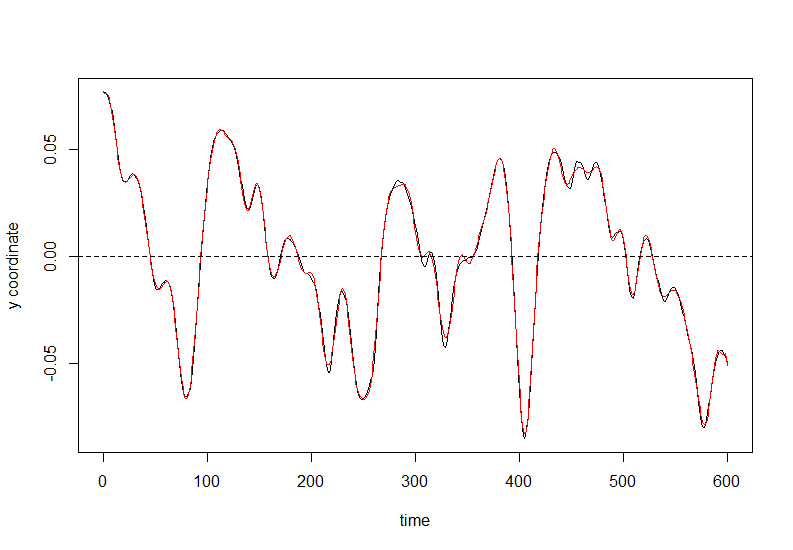
\includegraphics[scale=0.7]{fp03.png}\\
The black curve is original data and red curve is smoothed function using bspline system with 80 basis functions.\\
Then calculate the derivatives of both and combine the derivatives using
$$
speed=\sqrt{(f'(x))^2+(f'(y))^2}
$$
speed was adjusted by shifting the x axis by -1 to avoid detrimental numerical errors.\\
The results of single speed curve is as followed.\\
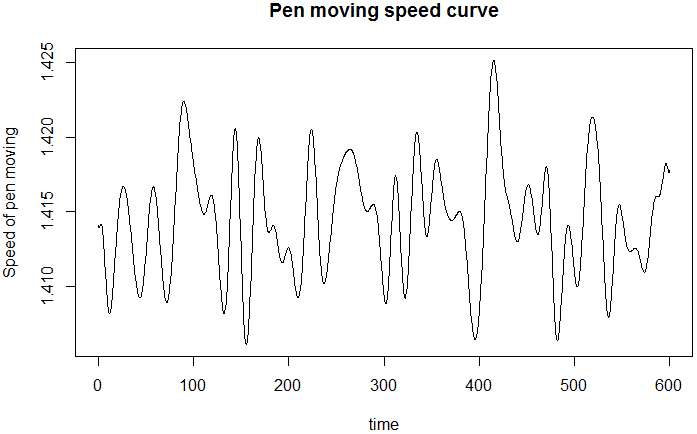
\includegraphics[scale=0.7]{fp04.png}\\
If we plot all 50 curves together we got\\
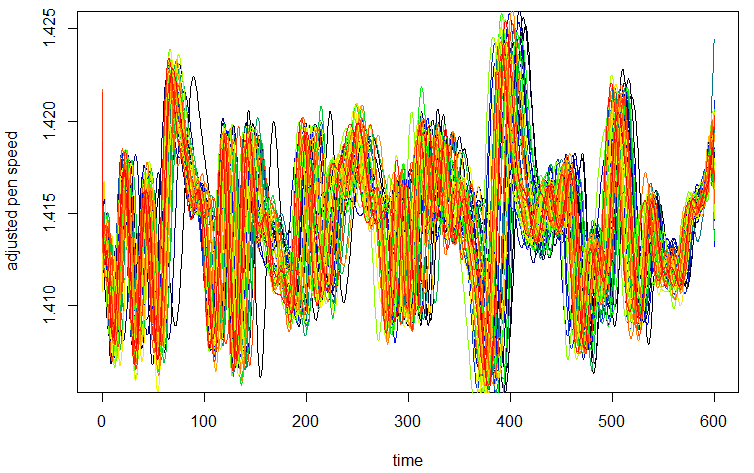
\includegraphics[scale=0.7]{fp02.png}\\
as you can see that they kind of share similar patterns, but the features(peaks and valleys) are shifted from each other. Thus our main goal here is to register those curves. In order to facilitate following analysis like regression and analysis of variance.\\

\bigskip

3. Registration\\
In this project, we will use SRSF method to register functions. And we will calculate the matrix of amplitude difference da and phase difference dp.\\
Firstly, we need to convert all the functions to q form by using formula
$$
q=sign(f'(x))\sqrt{|f'(x)|}$$
The following is q representation of first observation\\
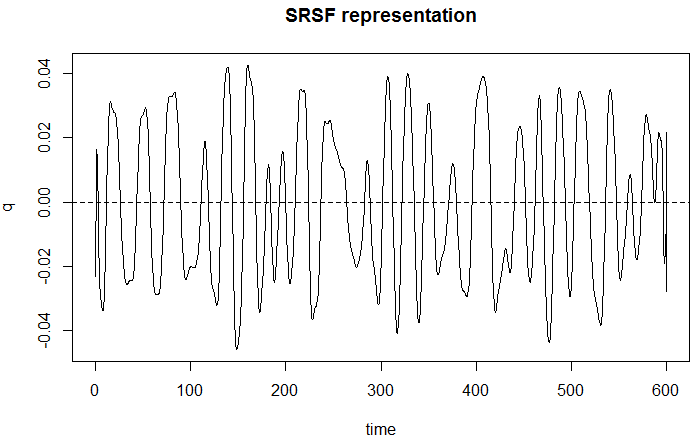
\includegraphics[scale=0.7]{fp05.png}\\
So I planed to register all 50 curves to their mean, however, it will not work because as showed in the following plot\\
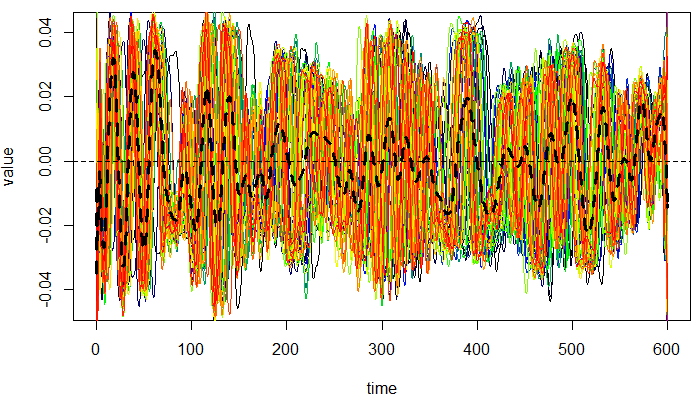
\includegraphics[scale=0.7]{fp06.png}\\
As shown in the above plot that the black dashed line is the mean curve. As you can see that the mean curve has lost lots of features because of phase difference and many of our peaks and valleys from different curves canceled each other. So we will register all 49 curves to the first observation.\\
Registration has been done by dynamic programming.\\
The first two curve has been registered very well as showed below\\
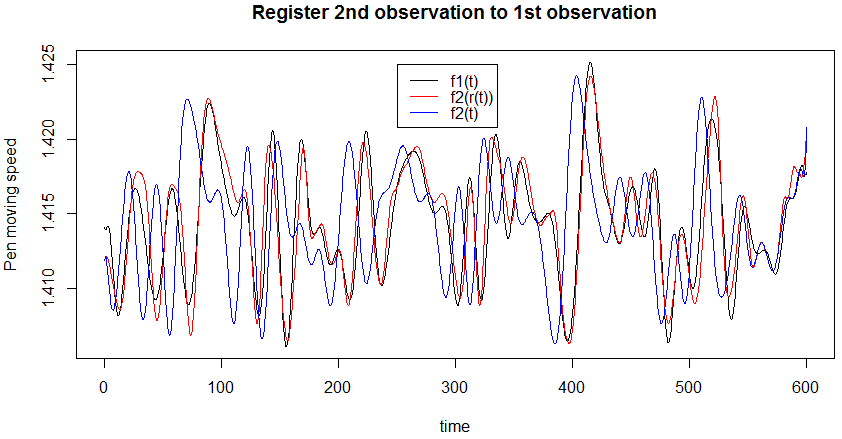
\includegraphics[scale=0.7]{fp07.png}\\
Phase difference is calculated by
$$
dp(f_1,f_2)=cos^{-1}(\int_0^1\sqrt{\gamma'(t)}dt)
$$
Amplitude difference is calculated by
$$
da(f_1,f_2)=\inf_{\gamma \in \Gamma}(||(f1,\gamma)-(f2,\gamma)||)
$$
After registration, 50 curves are shown below\\
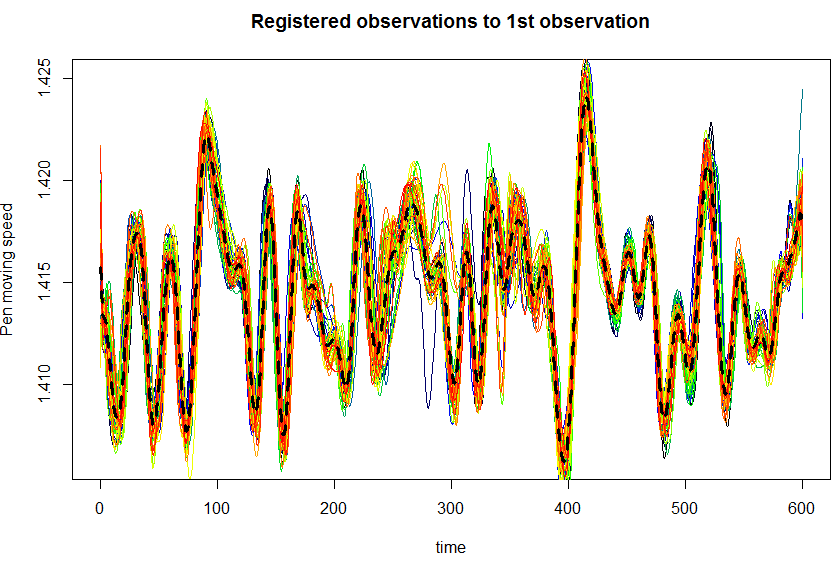
\includegraphics[scale=0.7]{fp08.png}\\
And da and dp are shown\\
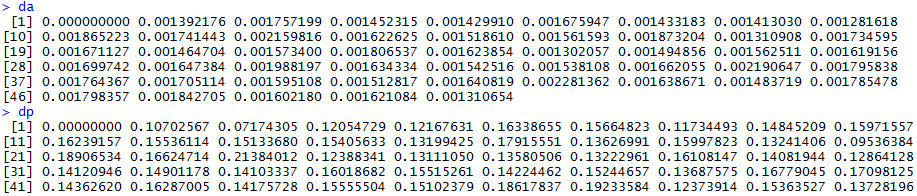
\includegraphics[scale=0.7]{fp09.png}\\
This is much nicer plot comparing to previous un-registrated one, with most of the peak and valleys distinct. And now we can see the mean curve make a lot more sense representing most of, if not all the features from these curves. \\

Finally, I made a animation of how the words was written along the 6 seconds, along the progressing of the pen moving speed. See. We can easily see that each peak is a stroke. So this data might be important for us to recognize hand-writing and identify signatures.\\
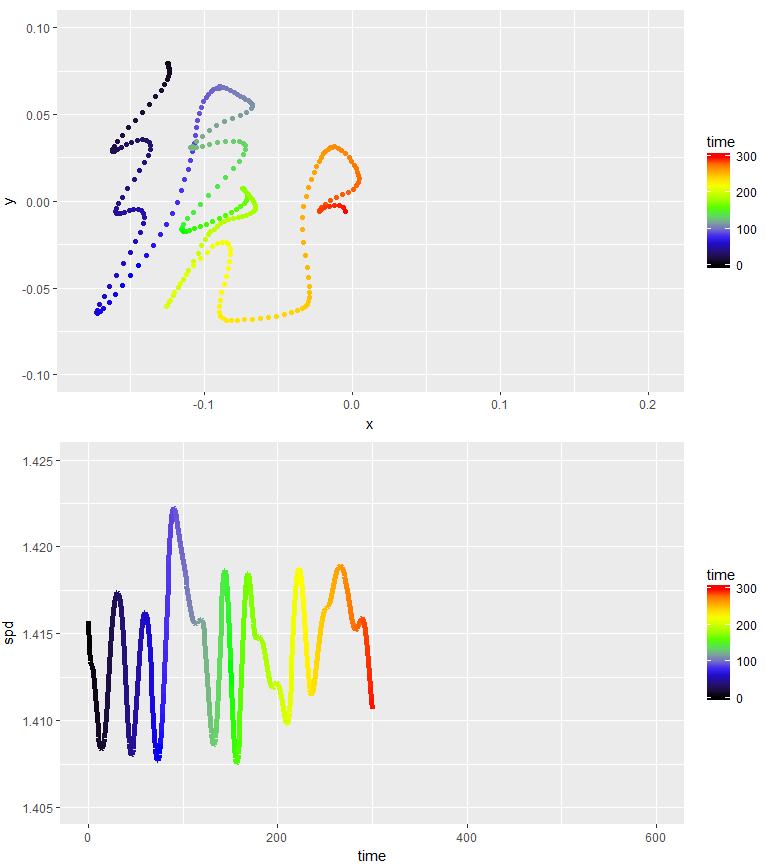
\includegraphics[scale=0.5]{fp010.png}\\

\bigskip

All code please see https://github.com/rikku1983/STAT5376\\
\bigskip

Thanks!


\end{document}